\documentclass[11pt]{article}

\usepackage[backend=bibtex]{biblatex}
\usepackage[utf8]{inputenc}
\usepackage{amsmath}
\usepackage{amssymb}
\usepackage{anysize}
\usepackage{graphicx}
\graphicspath{ {./images/} }
\usepackage{color}
\usepackage{xcolor}
\usepackage{algorithm2e}
\usepackage{pgfplots}
\usepackage{hyperref}
\usepackage{booktabs}
\bibliography{bibliography.bib}

\usepackage{tikz}
\usetikzlibrary{shapes,arrows}

\definecolor{mygreen}{rgb}{0,0.6,0}
\definecolor{mygray}{rgb}{0.5,0.5,0.5}
\definecolor{mypurple}{rgb}{0.58,0,0.82}

\usepackage{listings}

\usepackage{caption}
\DeclareCaptionFont{white}{\color{white}}
\DeclareCaptionFormat{listing}{\colorbox{gray}{\parbox[c]{\textwidth}{#1#2#3}}}

\setlength\parindent{0pt}
\setlength{\parskip}{10pt}

\marginsize{2cm}{2cm}{1cm}{1cm}

\usepackage{titlesec}
\titleformat{\section}{\large\bfseries}{\thesection}{1em}{}

\begin{document}

%  Title and authors
   \begin{center}
     {\huge\bfseries B31XP Robotics project\\ Robotic object follower}\\
      \vspace{2ex}
      \textsc{Andrey Pak, Donatas Kozlovskis, Enric Cornellà,\\ Fernando Garcia,  Igor Peric}
   \end{center}
   \vspace{2ex}%

%  Abstract
\begin{abstract}
This project presents a small, easy to build low-cost robot system, that is able to find coloured signs on the floor and implement the associated actions, e.g. stop, turn, pause, etc.
The robot hardware uses Raspberry Pi to control a set of motors, sensors and servo actuators. 
Report provides information about done review the hardware design and implementation of software using open source tools as C++ and OpenCV libraries. 
\end{abstract}
 
%%%%%%%%%%%%%%%%%%%%%%%%%%%%%
\section{Software}


Conceptual overview of software architecture and its parts is given on figure below. All components will be discussed and described in detail in this section of the report. 

\begin{figure}[th!]
\center
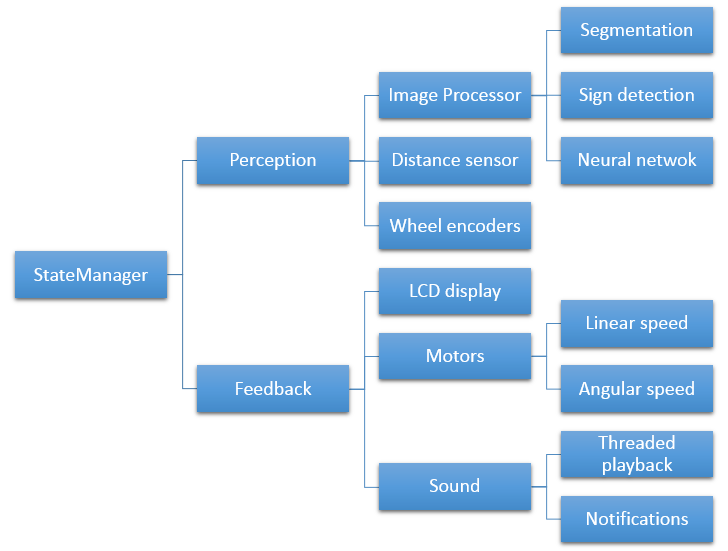
\includegraphics[scale=0.7]{images/software-architecture.png}
\caption{Overview of software architecture of the solution}
\end{figure}




\section{State machine}


One of the most common and intuitive approaches for implementation of software controller for hardware system is state-machine approach. It is fairly simple concept, with only a couple of important considerations.

System controlled by state machine has certain number of possible, unique and well defined states that it can be in at every moment of execution. State defines the behaviour of the system in every discrete moment of time, including three important aspects: sensor data acquisition, output behaviour computation and state transition check. In other words, every state has it is own logic for doing all of these three mentioned steps, which gives a lot of variability for possible control scenarios. It is worth mentioning that some states might skip certain steps or perform some steps more than once without state transition check, for example.

\paragraph{System states}

At any moment of time robot can be in one of the following state:

\begin{itemize}
	\item IDLE
	\item WIGGLING
	\item APPROACHING\_SIGN
	\item EXECUTING\_COMMAND
	\item MARCHING\_FORWARD
	\item GAME\_OVER 
\end{itemize}

\textbf{IDLE} state sets both angular and linear speed to zero and waits for any of the segmented object currently inside view to go away, after which it goes to WIGGLING state.

\textbf{WIGGLING} state rotates the robot around its vertical axis with constant angular and zero linear speed until a sign is detected. After detecting a sign it switches to APPROACHING\_SIGN state.

\textbf{APPROACHING\_SIGN} state moves the robot close to the sign it has seen in the previous state. It does this by setting the linear speed to constant value and adjusting angular speed all the time based on the horizontal position of the target sign in the view. Robot will move in the direction needed to align the sign to the center of the screen, and it will do that proportionally to the distance of the target to the center.

\textbf{EXECUTING\_COMMAND} state has different behavior depending on the type of the sign that was seen in the state before. If it was goal sign, it will switch to the GAME\_OVER state and the game will end. If it was stop sign, robot will just wait for certain predefined time-out (5 seconds) and switch to state MARCHING\_FORWARD. If it was the arrow sign, robot will turn desired angle and switch switch to state MARCHING\_FORWARD.

\textbf{MARCHING\_FORWARD} state sets the linear speed to constant and angular to zero. In this state robot constantly monitors camera image stream and can potentially switch to APPROACHING\_SIGN state once a sign is detected in perceptive area of the image.

\textbf{GAME\_OVER} state is entered after goal sign is approached. After displacing notification about game completion (through audio and visual feedback), robot remains idle until hardware button is pressed for the start of the new game.

\begin{figure}[th!]
	\centering
	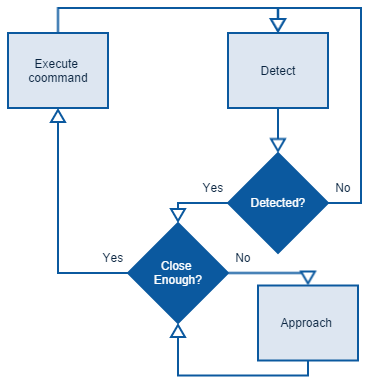
\includegraphics[scale=1]{algorithm-diagram.png}
	\caption{State transition algorithm}
	\label{fig:algorithm-diagram}
\end{figure}

\paragraph{Sensor data acquisition}

First step in state machine control loop is sensor acquisition step. If possible, data is acquired from all input sensors in order to determine current state of the environment. This includes acquisition of camera image using OpenCV, reading heading angle from motor driver and reading distances from ultrasonic sensor driver.

Last values of all the readings are always stored in local members of the class, so they can be referenced between successive acquisitions.

\paragraph{Output behavior computation}

Based on the sensed input data values for all output units are being calculated. This includes linear and angular wheel velocities, message for LCD display, sound to be played on speakers, etc.

\paragraph{State transition condition}

Every state has to have clearly defined condition which will make the system switch to any of the other states. System remains in the current state until one of the state transition conditions has been met.





%%%%%%%%%%%%%%%%%%%%%%%%%%%%%
\section{Vision module}


The task of vision subsystem is to handle the image data acquired from Raspbery Pi camera. This handling includes two basic subtasks: sign detection and sign recognition (classification).

Three basic signs detected and recognized by the system are shown on figure \ref{fig:raw-signs}. They are printed on a flat paper surface.

\begin{figure}[th!]
	\centering
	\begin{subfigure}[b]{0.2\textwidth}
		\centering
		
\includegraphics[scale=0.25]{sign-circle.png}
		\subcaption{Circle (goal)}
	\end{subfigure}
	\begin{subfigure}[b]{0.4\textwidth}
		\centering
		
\includegraphics[scale=0.25]{sign-arrow.png}
		\subcaption{Arrow (direction change)}
	\end{subfigure}
	\begin{subfigure}[b]{0.2\textwidth}
		\centering
		
\includegraphics[scale=0.25]{sign-cross.png}
		\subcaption{Cross (stop)}
	\end{subfigure}
	\caption{Shape of signs used by the system}
	\label{fig:raw-signs}
\end{figure}

Basic workflow of the vision processing module is split into functional blocks, shown on the figure \ref{fig:vision-module-blocks}.

%\begin{figure}[th!]
%	\centering
%		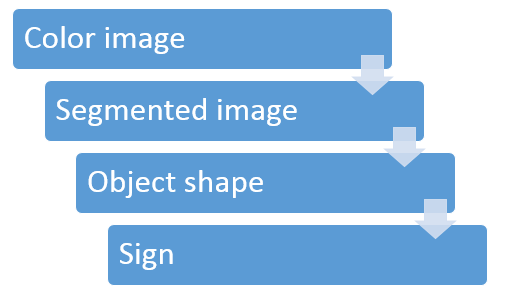
\includegraphics[scale=0.5]{image-module.png}
%	\caption{Workflow of vision module}
%	\label{fig:vision-module-blocks}
%\end{figure}

\begin{figure}[!ht]
	\centering
	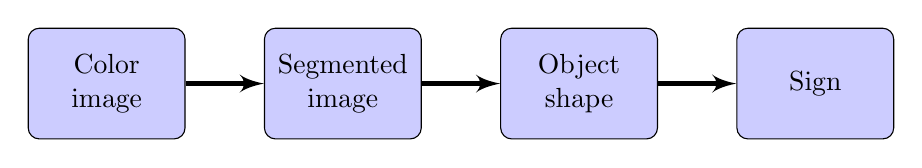
\begin{tikzpicture}[node distance = 2cm, auto]
	\tikzstyle{block} = [rectangle, draw, fill=blue!20, 
	text width=5em, text centered, rounded corners, minimum height=4em]
	\tikzstyle{line} = [draw, -latex', line width =2pt]
	% Place nodes
	\node [block] (ci) {Color image};
	\node [block, right of=ci, node distance = 3 cm] (si) {Segmented image};
	\node [block, right of=si, node distance = 3 cm] (os) {Object shape};
	\node [block, right of=os, node distance = 3 cm] (sign) {Sign};
	% Draw edges
	\path [line] (ci) -- (si);
	\path [line] (si) -- (os);
	\path [line] (os) -- (sign);
	\end{tikzpicture}
	\caption{Workflow of vision module}
	\label{fig:vision-module-blocks}
\end{figure}




Different methods and challenges encountered in vision module are described and discussed separately in the following chapters of the report.
\paragraph{Inverse Perspective Mapping}

In this project, a single camera mounted in the front of the robot with small tilting angle is used to capture the images. Since object of interest are found on a ground plane, before applying any image recognition and classification methods, it is common-sense to process obtained camera images using Inverse Perspective Mapping (IPM).
Knowing that camera tilting angle and position on the robot is fixed, this transform is just a  plane-to-plane homography to convert the perspective image to
top view to the ground plane image. The IPM can be applied to all three planes of colour image separately or only on selected colour plane. Example of the transform can be seen in figure \ref{fig:ipm_example}.
\begin{figure}[!ht]
	\centering
	\begin{subfigure}[b]{0.3\textwidth}
		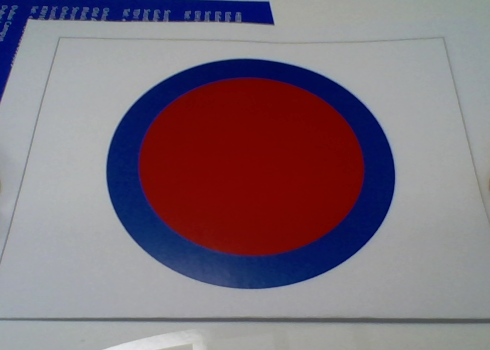
\includegraphics[width = 1\textwidth]{invPersInput.png}
		\caption{Robot captured image}
		\label{fig:}
	\end{subfigure}%
	~ 
	\begin{subfigure}[b]{0.3\textwidth}
		
\includegraphics[width = 1\textwidth]{invPersOutput.png}
		\caption{Output image after IPM}
		\label{fig:}
	\end{subfigure}
	%main caption
	\caption{Example of Inverse Perspective Mapping on a single colour image plane}
	\label{fig:ipm_example}
\end{figure}

\paragraph{Thresholding}

The first and the most intuitive approach to sign detection procedure was simple color thresholding, since signs which had to be detected are purely red.

The initial choice for color thresholding was HSV color space. Ranges of H (hue), S (saturation) and V (value) channels are [0,180], [0, 255] and [0, 255], respectively. In order to segment only red color, values of H (hue) channel greater than 170 and lower than 10 were used, since this range represents the band of red color. Additionally, too dark (V $ < $ 40), to bright (V $ > $ 220) and non-saturated pixels (S $ < $ 40) were rejected to improve the quality of segmentation. Results are shown on the figure ~\ref{fig:color-spaces}.

\begin{figure}[th!]
	\centering
	\begin{subfigure}[b]{0.3\textwidth}
		\centering
	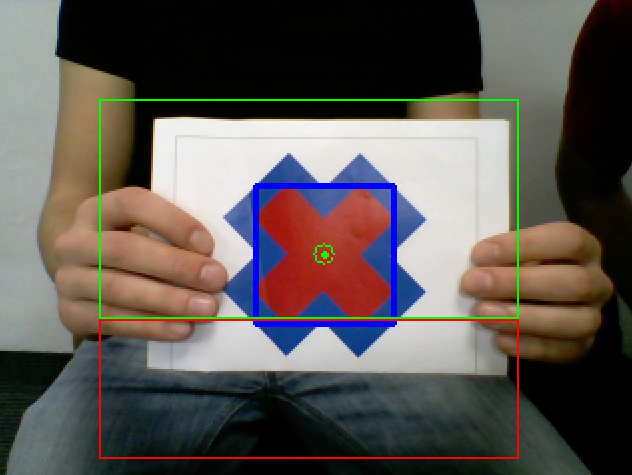
\includegraphics[scale=0.33]{thresholding-raw.png}
	\subcaption{Raw camera input}
	\end{subfigure}
	\begin{subfigure}[b]{0.3\textwidth}
		\centering
		
\includegraphics[scale=0.7]{thresholding-hsv.png}
		\subcaption{HSV color space}
	\end{subfigure}
	\begin{subfigure}[b]{0.3\textwidth}
		\centering
		\includegraphics[scale=0.7]{thresholding-YCrCb.png}
		\subcaption{YCrCb color space}
	\end{subfigure}
	\caption{Comparison of color spaces used for thresholding}
	\label{fig:color-spaces}
\end{figure}

After some testing, YCrCb color space proved to give better results for segmentation, as shown on figure above. As a result, YCrCb colour space was used in final implementation.

Usage of IR camera did not affect the recognition quality of the thresholding procedure in regular, normal lighting conditions. On the other hand, it drastically increased the accuracy in low lighting conditions, which is described in Hardware section of the report.

The biggest connected component (blob) in the thresholded image is considered to be a sign. Bounding box of the biggest blob determined the area of the thresholded image to be passed in as an input to the sign classification module. 

\paragraph{Classification of the signs using statistical moments}

Taking into consideration the relatively low computational power of the hardware platform used to develop the system, priority for the chosen sign classification algorithm was low complexity.

After some thorough analysis of the available option, statistical moments proven to be the best option.

For an arbitrary binary (i.e. thresholded) input image system can compute statistical moments of desired order. The moment of importance in case of sign classification was center of mass or first order moment. It can be thought of average coordinate of all white pixels for both axes.

\begin{figure}[th!]
	\centering
	\begin{subfigure}[b]{0.25\textwidth}
		\centering
		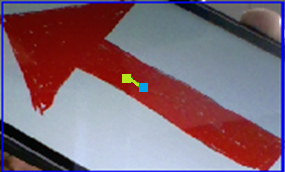
\includegraphics[scale=0.55]{moments-arrow-raw.png}
		\subcaption{Raw camera input}
	\end{subfigure}
	\begin{subfigure}[b]{0.25\textwidth}
		\centering
		
\includegraphics[scale=0.8]{moments-arrow-segm.png}
		\subcaption{Arrow}
	\end{subfigure}
	\begin{subfigure}[b]{0.2\textwidth}
		\centering
		
\includegraphics[scale=0.8]{moments-cross-segm.png}
		\subcaption{Cross}
	\end{subfigure}
	\begin{subfigure}[b]{0.2\textwidth}
		\centering
		
\includegraphics[scale=0.9]{moments-circle-segm.png}
		\subcaption{Circle}
	\end{subfigure}
	\caption{Visual cues for sign classification using statistical moments}
	\label{fig:statistical-moments}
\end{figure}

Figure \ref{fig:statistical-moments} demonstrates intuition behind visual cues used for discrimination of three different types of signs. By computing the distance of center of the mass (green rectangle) and center of the cropped image segment where the sign was detected (blue rectangle) we can perform initial discrimination between \textbf{arrow} and \textbf{rest two signs}. Distance is going to be close to zero in case of cross and circle since object are symmetrical around two mutually normal axes. Arrow is not symmetrical around one axis, so it's center of the mass will be slightly shifter towards the tip of the arrow and this is the property used to distinguish an arrow from the circle and cross.
Table \ref{tab:moments} shows average distance of center of the mass from image center proportional to cropped image size. Clear observation is that thresholding this distance to 10 $\%$ can give is pretty good estimate of probability that sign belongs to arrow class.

If this distance is close to zero, additional step is needed to determine is the observed sign cross or circle. Approach used in this step was investigation of zero-order moment, which gives the number of white pixels in the image. By taking the ratio of zero order moment and total number of pixels of sign area, we can distinguish between cross and circle. Intuition behind this metric lies in the fact that circle has bigger surface than cross of the same bounding box size, so the percentage of space it occupies in the cropped image area where the sign is going to be larger than if it was cross. Table \ref{tab:moments} gives suitable value of threshold of 70 $\%$.

\begin{table}[th!]
\centering
\begin{tabular}{l*{2}{c}r}
	Sign class			& Distance of first moment & Ratio of second order moment  \\
	\hline
	Arrow 				& 18.41 & 56.44  \\
	Cross            	& 1.39 & 54.20  \\
	Circle           	& 0.97 & 89.63  \\
\end{tabular}
\caption{Numerical values of statistical moments given in $\%$ wrt. image size}
\label{tab:moments}
\end{table}

Described method proved to be sufficiently accurate for practical purposes, while still remaining \textbf{computationally tractable} on available hardware. More robust classification methods will be discussed in section \ref{sec:future-improvements} and are subject to future investigation.

\paragraph{Neural network classifier}

Justification of usage neural networks.

Very brief theoretical background.

Description of the way how we train it on images (raw pixel values, segmentation pixels, hu-moments as inputs, etc)

Description of tested recognition method (sliding window, random, ...)

Performance comparison with previous method.

\paragraph{Computing arrow orientation}

After sign has been classified as arrow, additional step needs to be performed in order to extract the arrow angle relative to the orientation of the robot at the moment of observation.

Initial idea was to use already computed information about the statistical moments to get the orientation of the arrow. Center of the mass and center of the cropped image segment containing the sign form a vector pointing towards tip of the arrow. We can exploit this information to determine the angle of the vector, as shown on figure \ref{fig:arrow-angle-computation}. Although not so robust, this was intuitive and the fastest method to prototype since all moments are already computed for sign classification step, which meant that this method would reduce computational overhead.

\begin{figure}[th!]
	\centering
	\begin{subfigure}[b]{0.45\textwidth}
		\centering
		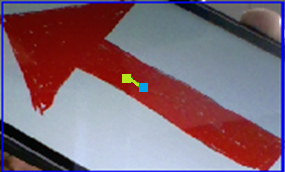
\includegraphics[scale=0.7]{moments-arrow-raw.png}
		\subcaption{Raw camera input}
	\end{subfigure}
	\begin{subfigure}[b]{0.45\textwidth}
		\centering
		
\includegraphics[scale=1]{moments-arrow-segm-angle.png}
		\subcaption{Arrow}
	\end{subfigure}
		\begin{subfigure}[b]{0.45\textwidth}
			\centering
			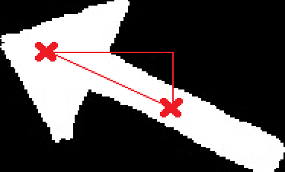
\includegraphics[scale=0.7]{moments-arrow-segm-angle-math.png}
			\subcaption{Angle from moments}
		\end{subfigure}
		\begin{subfigure}[b]{0.45\textwidth}
			\centering
			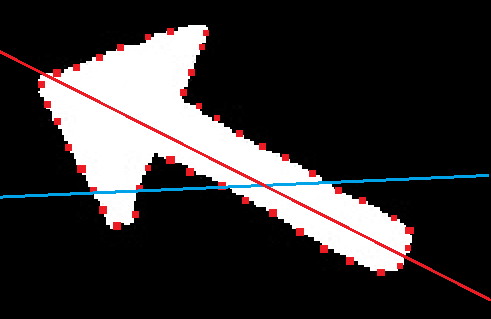
\includegraphics[scale=0.55]{moments-arrow-segm-angle-fitting.png}
			\subcaption{Line fitting}
			\label{fig:line-fitting}
		\end{subfigure}
	\caption{Computation of the arrow orientation}
	\label{fig:arrow-angle-computation}
\end{figure}

After implementation and extensive testing of mentioned method, some scenarios where it fails were met. One of them is shown in the figure , where wrong value of the angle is computed or it wasn't reliable enough (it was oscillating a lot). Oscillation problem could have been solved by filtering, but instead a different approach was chosen.

Instead of focusing on statistical properties of the contour of the arrow better approach is to utilize the whole information about it's contour. Contour of the arrow shape is extracted from segmented binary image of the arrow. Array of points representing the contour is then fitted to the line in \textbf{Linear Least Squares fashion (LLS)}, which is a well known function minimization framework for linear systems.

The basic idea is posing the problem of finding unknown arrow angle $\theta$ as function minimization problem, where input is defined as set $C$ of $N$ contour points $C_i \in \mathbb{R}^2$. Cost function on a set of points $C$ and chosen angle $\theta$ is defined as sum of the squared distance of each contour point $C_i$ from the line with angle $\theta$, which is formally given by equation \ref{eq:LLS}. Minimizing this function over $\theta$ gives the optimal line angle that fits the given contour points.

\begin{equation}
f(C,\theta)=
\frac{1}{N}
\sum_{i=1}^{N}distance(C_i, line(\theta))^2
\label{eq:LLS}
\end{equation}

Figure \ref{fig:line-fitting} shows two arbitrary lines on top of the segmented image of the arrow. Blue line has higher value of the cost function than the red line because it doesn't fit the given data (contour points) the best possible way. Red line is the optimal angle for given shape, determined by least square solution of the equation \ref{eq:LLS}.

OpenCV has LLS implementation of described line fitting algorithm, which was used in the final version of the solution. Using this method improved the accuracy and stability of orientation of the arrow without significant impact on performance, since optimization problem can be solved using techniques linear algebra, which are computationally inexpensive.

\paragraph{Solving partial occlusion and re-detection}

Problem of partial occlusion arises when robot is moving forward and a sign is slowly getting into the area observed by robot. Some time is needed before the sign completely enters the view and attempt of classification partially visible sign would result in misclassification in most of te cases.

Also, there is a problem of detecting proximity of the robot to the observed sign, because desired behavior is to switch states only when the robot is close to sign it detects and not as soon it detects it.

In order to prevent attempts of classifications of partially visible signs and detecting proximity of the robot to the sign, whole view of the camera is split into two regions of interest: \textbf{perceptive area} and \textbf{proximity area}, shown on figure \ref{fig:camera-view-areas}. Using these view areas system is able to overcome the described problems in very easy and intuitive way.

\begin{figure}[th!]
	\centering
		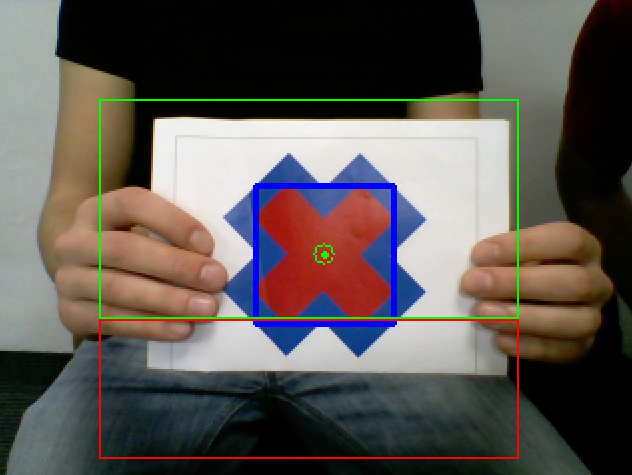
\includegraphics[scale=0.5]{thresholding-raw.png}
	\caption{Perceptive (green) and proximity (red) area}
	\label{fig:camera-view-areas}
\end{figure}

Detection of the sign (segmentation and blob detection) are performed at every iteration and position of the object is extracted as center of the detected blob. For predefined camera position and physical size of the signs, it can be assumed that \textbf{if object's center is inside the perception area it will be completely inside the camera view}. This allows reliable determination of exact classification moment, without risk of classifying partially visible objects.

Similar strategy is used for detecting the proximity of the sign: if it's center is in the proximity area it is assumed to be close to the robot. Since slightly delayed image processing and low FPS, it will take some time for robot to determine that it approached the sign. This will result in robot ending up exactly on the sign at the moment when it switches to execution of the command defined by the sign.


\section{Further improvements}


\subsection{Robustness of sign classification}

Current sign classification approach is computationally inexpensive and has a simple implementation and execution. It results in low robustness, meaning that on some occasions the robot detects some other red object's shape as one of the three signs that it needs to classify.

In order to avoid these issues, a more robust classifier is required. An approach using artificial neural networks, Support Vector Machines or any other machine learning technique would require training classifiers on another (more powerful) CPU and loading the trained classifier to the robot just for the purpose of classification.

\subsection{Complex game rules and sign diversity}

Current rules for interaction with robot rely only on a couple of simple actions and available signs. Software control architecture is built in a modular way, which enables easy addition of the new signs under assumption of robust classifier able to distinguish between all currently known signs and newly added one.

Expanding set of available signs could enrich the game experience by introducing new objectives, goals and obstacles for the children to play with.

\subsection{Hardware improvements}

Although system is currently capable of performing all desired tasks, a more powerful processing hardware would make it faster, more responsive and funnier for children to play with. Having only 6 \textit{fps} from camera, limits the maximum speed of robot movement so games would look more dynamic if the robot were able to move faster. 
It would also enable usage of more advanced and, at the same time, more robust algorithms for image processing. This would remove some limitations and conditions put on the usage of the robot, like camera pointing only towards ground (floor) plane, maximum distance of sign placement, sign shape and colour restrictions, etc..
More sensors would enrich engagement of the children as well by providing diverse set of ways to interact with the robot. 




\clearpage


\end{document}